\section{Implemented use cases}

The following five use cases have been prototyped in the TenSyGrid Stability Monitor, a web-based graphical interface that communicates with the native Python TenSyGrid calculation engine (the ported MTI implementation integrated within VeraGrid), running on a dedicated backend server. 

% ---------------------------------------------------------------------------
\subsection{UC-01: Assessment of small-signal stability under given operating conditions}
% ---------------------------------------------------------------------------

\begin{description}
  \item[Actor.] Network operator or planning engineer.
  \item[Objective.] Load a grid model and compute its small-signal stability properties using the tensor-based multilinear formulation.
  \item[Preconditions.]
        \begin{itemize}[before=\leavevmode, leftmargin=*]
          \item The TenSyGrid engine backend is running and accessible via a web browser.
          \item At least one valid grid model is available. It may be supplied as a native \texttt{.veragrid} file, through any file format supported by VeraGrid's import layer, through the IPSA adapter from an external tool, or through a configured API endpoint.
          \item External adapters and API integrations must provide the topology, equipment parameters, operating point, and dynamic-model information required by the selected analysis, and the imported model must pass VeraGrid validation.
        \end{itemize}

  \item[Theoretical basis.] The iMTI formulation leads to the descriptor system $\mathbf{E}\dot{\mathbf{x}}=\mathbf{A}\mathbf{x}$, from which the generalized eigenvalue problem
        \[
          \lambda\mathbf{E}\mathbf{x}=\mathbf{A}\mathbf{x}
        \]
        is obtained. The solution provides the eigenvalues $\lambda=\sigma\pm j\omega$, where $\sigma$ governs decay/growth and $\omega$ the angular speed ($f=\omega/(2\pi)$). The damping ratio is $\zeta=-\sigma/\lvert\lambda\rvert$. In the tensor-based multilinear framework, the system matrices $\mathbf{S}$ and $\mathbf{\Phi}$ are assembled from the iMTI model, and the descriptor matrices $\mathbf{E}$ and $\mathbf{A}$ are constructed accordingly, from which the eigenpairs used in the subsequent analysis are derived~\cite{Kaufmann2025TenSyGridD11}.
  \item[Possible bottlenecks.] No multilinear implementation of a model yet~\cite{deJuanVela2026TenSyGridD33}. Scaling issues to be determined.
  \item[Main flow.]
        \begin{enumerate}[before=\leavevmode, leftmargin=*]
          \item The operator opens the \textbf{Run Analysis} tab.
          \item The input selector is populated with available grid-model files, IPSA-connected external sources, and configured API endpoints. The operator selects the desired source.
          \item The selected input is imported through the corresponding VeraGrid or IPSA adapter, validated, and converted into VeraGrid's internal \texttt{MultiCircuit} representation.
          \item The operator clicks the \textbf{Run Analysis} button.
          \item The backend launches the computational script as a subprocess, using the validated internal model and operating point as input.
          \item A log output panel displays the analysis progress: power-flow solution, state-matrix assembly, and eigenvalue computation.
          \item Upon completion, the result is stored as a \texttt{.tensygrid} file in the precomputed-results directory.
          \item The status indicator changes from \textit{Running} to \textit{Completed}, and the new result appears in the result list with a colour-coded stability badge (green: stable, yellow: marginal, red: unstable). A configurable numerical tolerance, currently $10^{-6}$ for the dominant real part, is used to distinguish a marginal result from numerical noise.
          \item If the operator needs to abort, the \textbf{Stop} button terminates the subprocess gracefully.
        \end{enumerate}

        \begin{figure}[H]
          \centering
          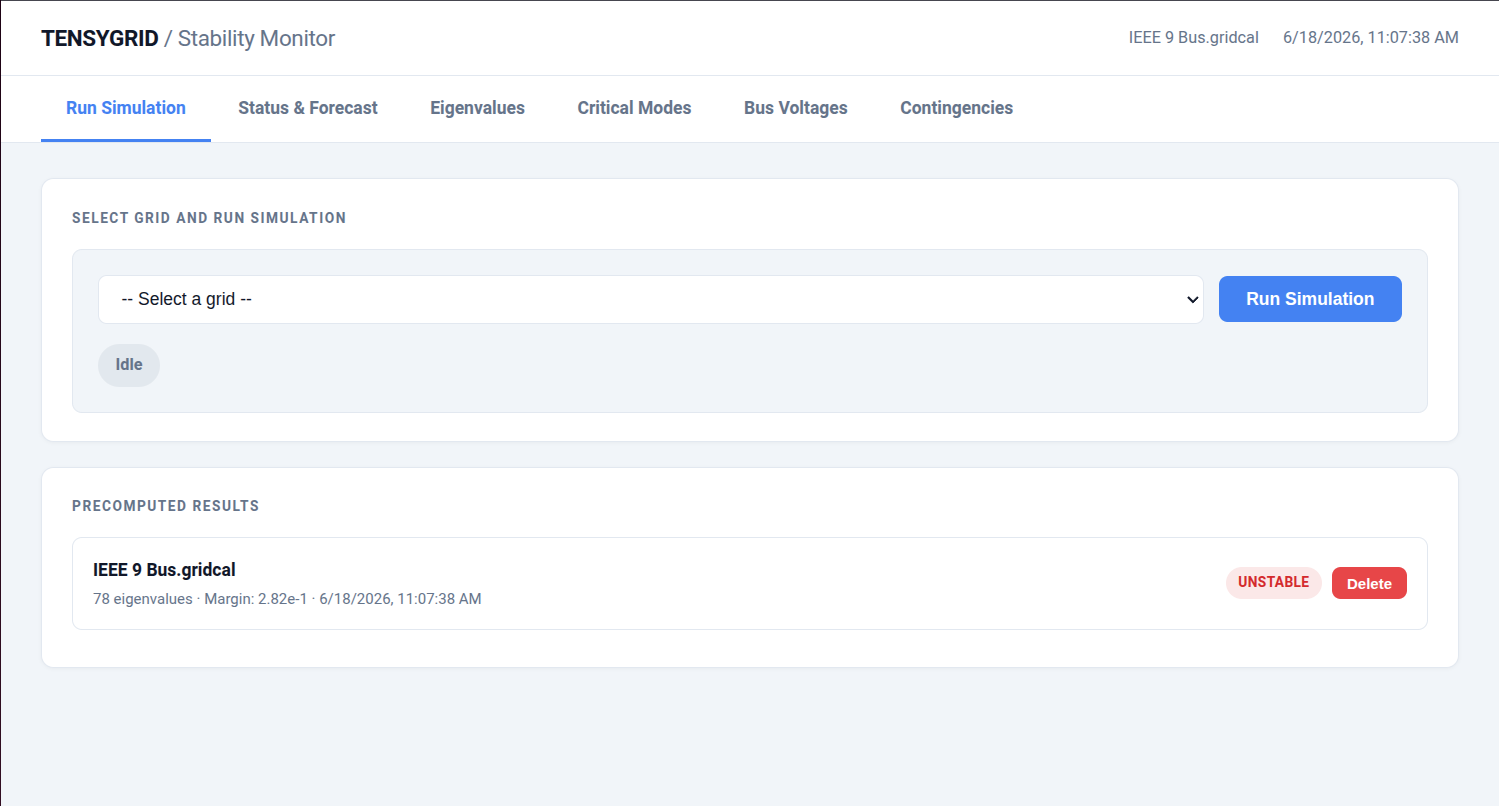
\includegraphics[width=0.7\textwidth]{pictures/UC-01.run_simulation.png}
          \caption[UC-01: Assessment of small-signal stability.]{UC-01: Assessment of small-signal stability under given operating conditions. The operator selects a grid model, runs the analysis, and monitors progress in the log panel. Upon completion, the result is stored and classified by stability status.}
        \end{figure}

  \item[GUI interaction.] The \textbf{Run Analysis} tab contains an input-source selector, action buttons (Run / Stop), a status badge, an execution log panel, and a list of previously computed results. File-based inputs display the detected format and any conversion warnings. IPSA and API-based sources additionally display connector status and validation results before the analysis starts. Each result item shows the analysis timestamp, the grid name, and the stability classification. A delete button allows removal of obsolete or failed results.
  \item[Expected result.] A \texttt{.tensygrid} file containing the full stability analysis output: eigenvalues, critical modes with participation factors, bus voltages from the power flow, grid topology information, the stability margin, and an operation hash for traceability. This file serves as input for all subsequent use cases (UC-02 to UC-05).
\end{description}




% ---------------------------------------------------------------------------
\subsection{UC-02: Monitoring and screening of power system small-signal stability margins}
% ---------------------------------------------------------------------------

\begin{description}
  \item[Actor.] Network operator; planning engineer or stability analyst for the detailed spectrum exploration.
  \item[Objective.] Obtain an immediate, general classification of grid stability together with key topological and operational metrics, and explore the full eigenvalue distribution in the complex plane to identify clusters, assess damping ratios, and detect modes of concern.
  \item[Preconditions.] At least one analysis (UC-01) has been completed and its result is loaded.
  \item[Theoretical basis.] Using UC-01 theoretical basis, we find different regimes in the system stability. We define the dominant eigenvalue $\lambda_1$ as the one with the biggest $\Re(\lambda)=\sigma$. For a sufficiently large time $t$, any other mode becomes negligible relative to the dominant one, since
        \[
          \frac{\mathrm{e}^{\lambda_n t}}{\mathrm{e}^{\lambda_1 t}}
          = \mathrm{e}^{(\lambda_n-\lambda_1)t} \xrightarrow[t\to\infty]{} 0 \quad \text{for } n\neq 1 \ \text{with } \sigma_1>\sigma_n .
        \]
        Therefore, if $\sigma_1>0$, the dominant term blows up to positive infinity, causing a clear instability, whereas $\sigma_1<0$ drives all modes to decay.

        These two verdicts are conclusive because, when no eigenvalue has $\Re(\lambda)=0$, the equilibrium is hyperbolic and the Hartman--Grobman theorem guarantees that, in a neighbourhood of the equilibrium, the nonlinear flow is topologically conjugate to its linearisation. The sign of $\sigma$ therefore reproduces the true local behaviour and not merely a first-order approximation. The theorem also marks the limit of the eigenvalue test: as soon as one mode reaches $\Re(\lambda)=0$, the equilibrium is non-hyperbolic, the linearisation is no longer topologically equivalent to the nonlinear flow, and the verdict has to come from higher-order terms (UC-13).

        The remaining singular case is a mode on the imaginary axis, $\Re(\lambda)=\sigma=0$, which may be a null eigenvalue ($\omega=0$) or a purely imaginary conjugate pair ($\lambda=\pm j\omega$, a Hopf-type mode): the argument above rests on the gap $\sigma_1-\sigma_n>0$, but here $\sigma_1=\sigma_n=0$ makes the exponent $\lambda_n-\lambda_1$ vanish, so the ratio does not tend to zero and the mode is not negligible relative to the dominant one. This equilibrium mode neither decays nor grows (it may oscillate with constant amplitude), i.e.\ a marginally stable regime that the dashboard classifies as \emph{yellow}.

        It is important, however, to distinguish this genuine marginal mode from spurious null eigenvalues that arise purely from the algebraic structure of the generalised eigenproblem $\lambda\mathbf{E}\mathbf{x}=\mathbf{A}\mathbf{x}$: whenever the leading matrix $\mathbf{E}$ (or the pencil $\lambda\mathbf{E}-\mathbf{A}$) is singular, the spectrum contains null eigenvalues that are not associated with any decaying, growing, or oscillating dynamic mode. These structural zeros must be identified and excluded before classifying the system, so that the \emph{yellow} verdict is reserved for actual marginal dynamics.

        In addition, each oscillation mode is represented by a conjugate pair of eigenvalues $\lambda=\sigma\pm j\omega$, where $\sigma$ governs decay-or-growth and $\omega$ the angular frequency, so that $f=\omega/(2\pi)$ is the frequency in Hz. In the complex plane, the ratio of $\sigma$ to $|\lambda|$ gives the damping ratio $\zeta=-\sigma/\lvert\lambda\rvert$, which equals the cosine of the mode's angle with the negative real axis: $\zeta=\cos\theta$. Constant-damping loci therefore appear as straight lines (cones) through the origin, which is precisely what the threshold lines used in the eigenvalue view (e.g.\ $\zeta=0$ and $\zeta=0.05$) represent. Modes close to the imaginary axis $\sigma\approx 0$ fall inside the low-damping cone and are flagged as the ones of concern; the spectrum is inspected to identify which modes concentrate the disturbance. This attribution, however, is the object of UC-03.
  \item[Possible bottlenecks.] To identify the origin of zero eigenvalues that lead to an inconclusive response.

  \item[Main flow.]
        \begin{enumerate}[before=\leavevmode, leftmargin=*]
          \item The operator navigates to the \textbf{Status} tab.
          \item A compact colour-coded badge displays the overall stability classification:
                \begin{itemize}[before=\leavevmode, leftmargin=*]
                  \item \textbf{Green} | Stable: all eigenvalues have negative real parts with sufficient damping.
                  \item \textbf{Yellow} | Marginal: the dominant real part lies within the configured numerical tolerance of the imaginary axis (currently $10^{-6}$), or some modes exhibit low damping ($\zeta < 0.05$).
                  \item \textbf{Red} | Unstable: at least one eigenvalue has a positive real part.
                \end{itemize}
          \item The \textbf{Grid Information} card shows the network topology: number of buses, generators, lines, loads, and transformers.
          \item The \textbf{Key Metrics} card reports the stability margin, the number of critical modes, the total eigenvalue count, and the number of state variables.
          \item A compact complex-plane eigenvalue plot provides a visual overview of the spectrum, with a red dashed line marking the stability boundary ($\Re(\lambda) = 0$).
          \item The \textbf{Stability Assessment} card presents a textual summary with colour-coded recommendations (e.g., ``All modes stable'', ``Caution: low damping detected'', or ``Warning: positive real parts; the system is unstable'').
          \item When a detailed exploration is required, the operator navigates to the \textbf{Eigenvalues} tab, where a full-page complex-plane scatter plot displays all eigenvalues: horizontal axis = real part $\sigma$, vertical axis = imaginary part $\omega$ (angular frequency). A red dashed vertical line marks the stability boundary ($\sigma = 0$).
          \item The operator can \textbf{scroll to zoom} and \textbf{drag to pan} across the plot, allowing inspection of dense clusters or outlying modes.
          \item Hovering over a point displays a tooltip with the eigenvalue's real part, imaginary part, frequency in Hz, and damping ratio $\zeta$.
          \item A \textbf{Damping vs.~Frequency} scatter plot shows $\zeta$ against frequency. Critical threshold lines at $\zeta = 0$ and $\zeta = 0.05$ are drawn for reference.
          \item A full \textbf{Eigenvalue Table} lists all eigenvalues in tabular form, sortable by real part, damping, or frequency.
          \item An \textbf{Info} button opens a modal overlay explaining how to interpret eigenvalue plots and damping ratios, targeted at operators who may not be familiar with small-signal analysis.
        \end{enumerate}

        \begin{figure}[H]
          \centering
          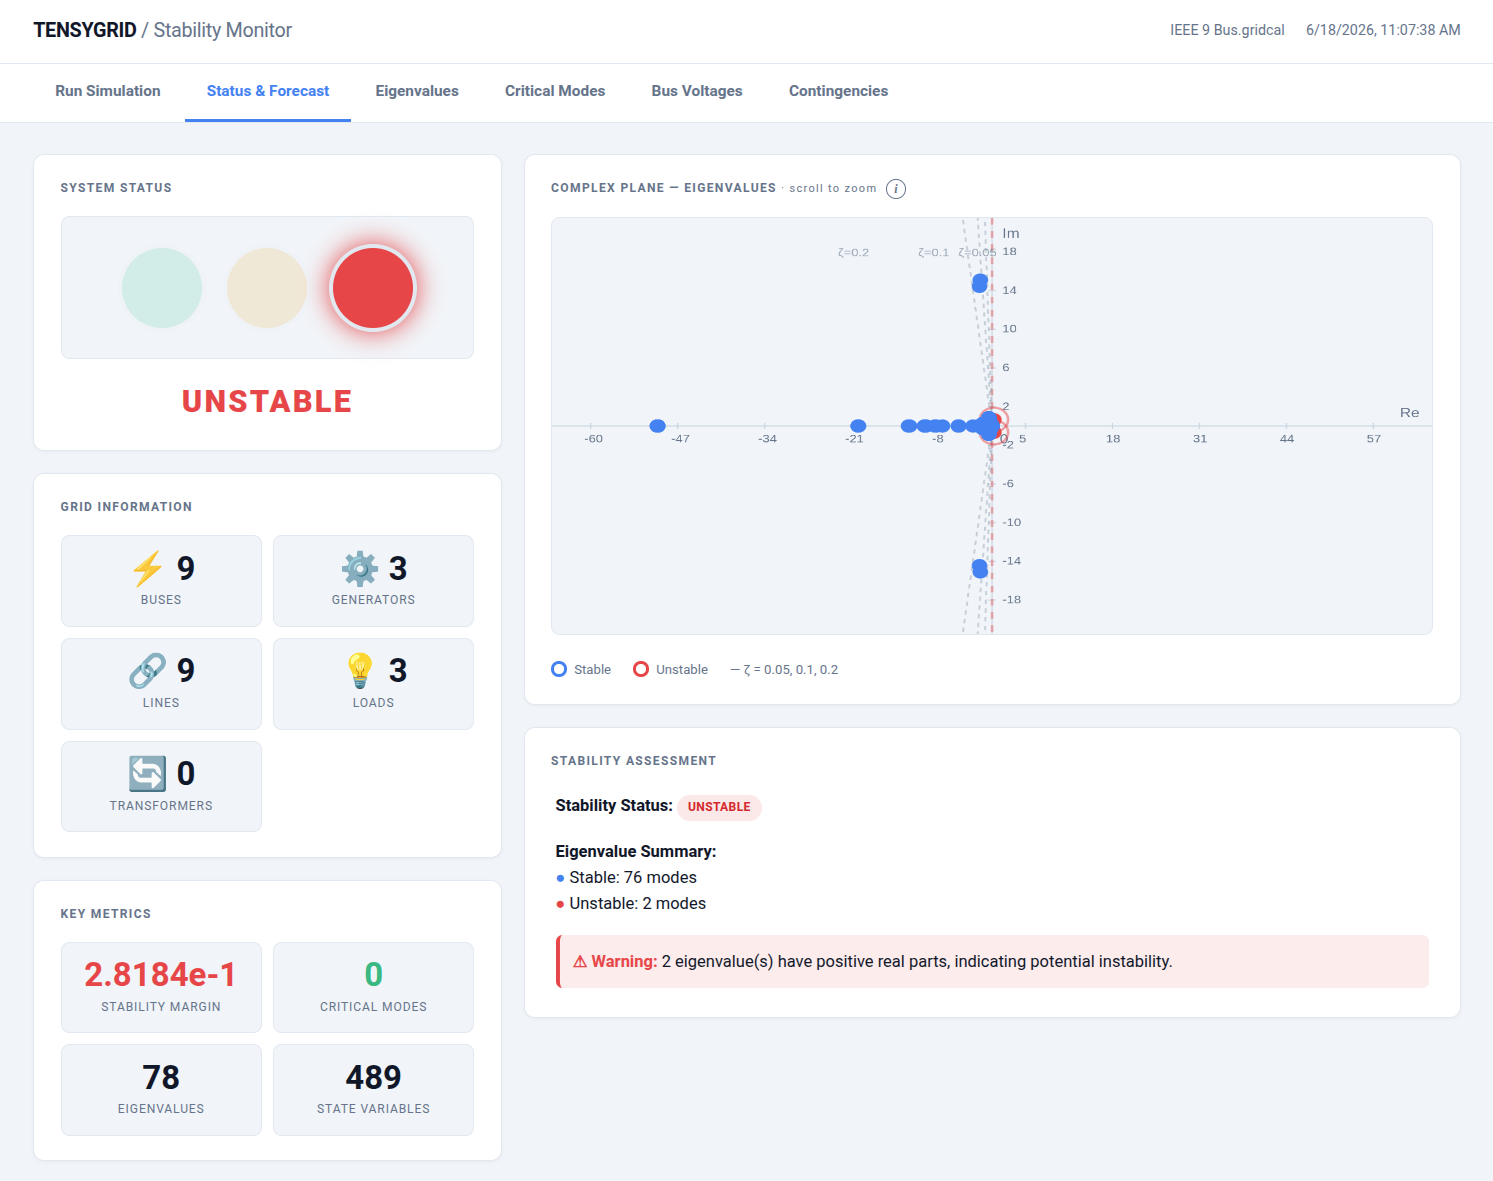
\includegraphics[width=0.7\textwidth]{pictures/UC-02.status_dashboard.png}
          \caption[UC-02: Status.]{UC-02: Status. The operator views the grid's stability status and related information in a consolidated dashboard.}
        \end{figure}

        \begin{figure}[H]
          \centering
          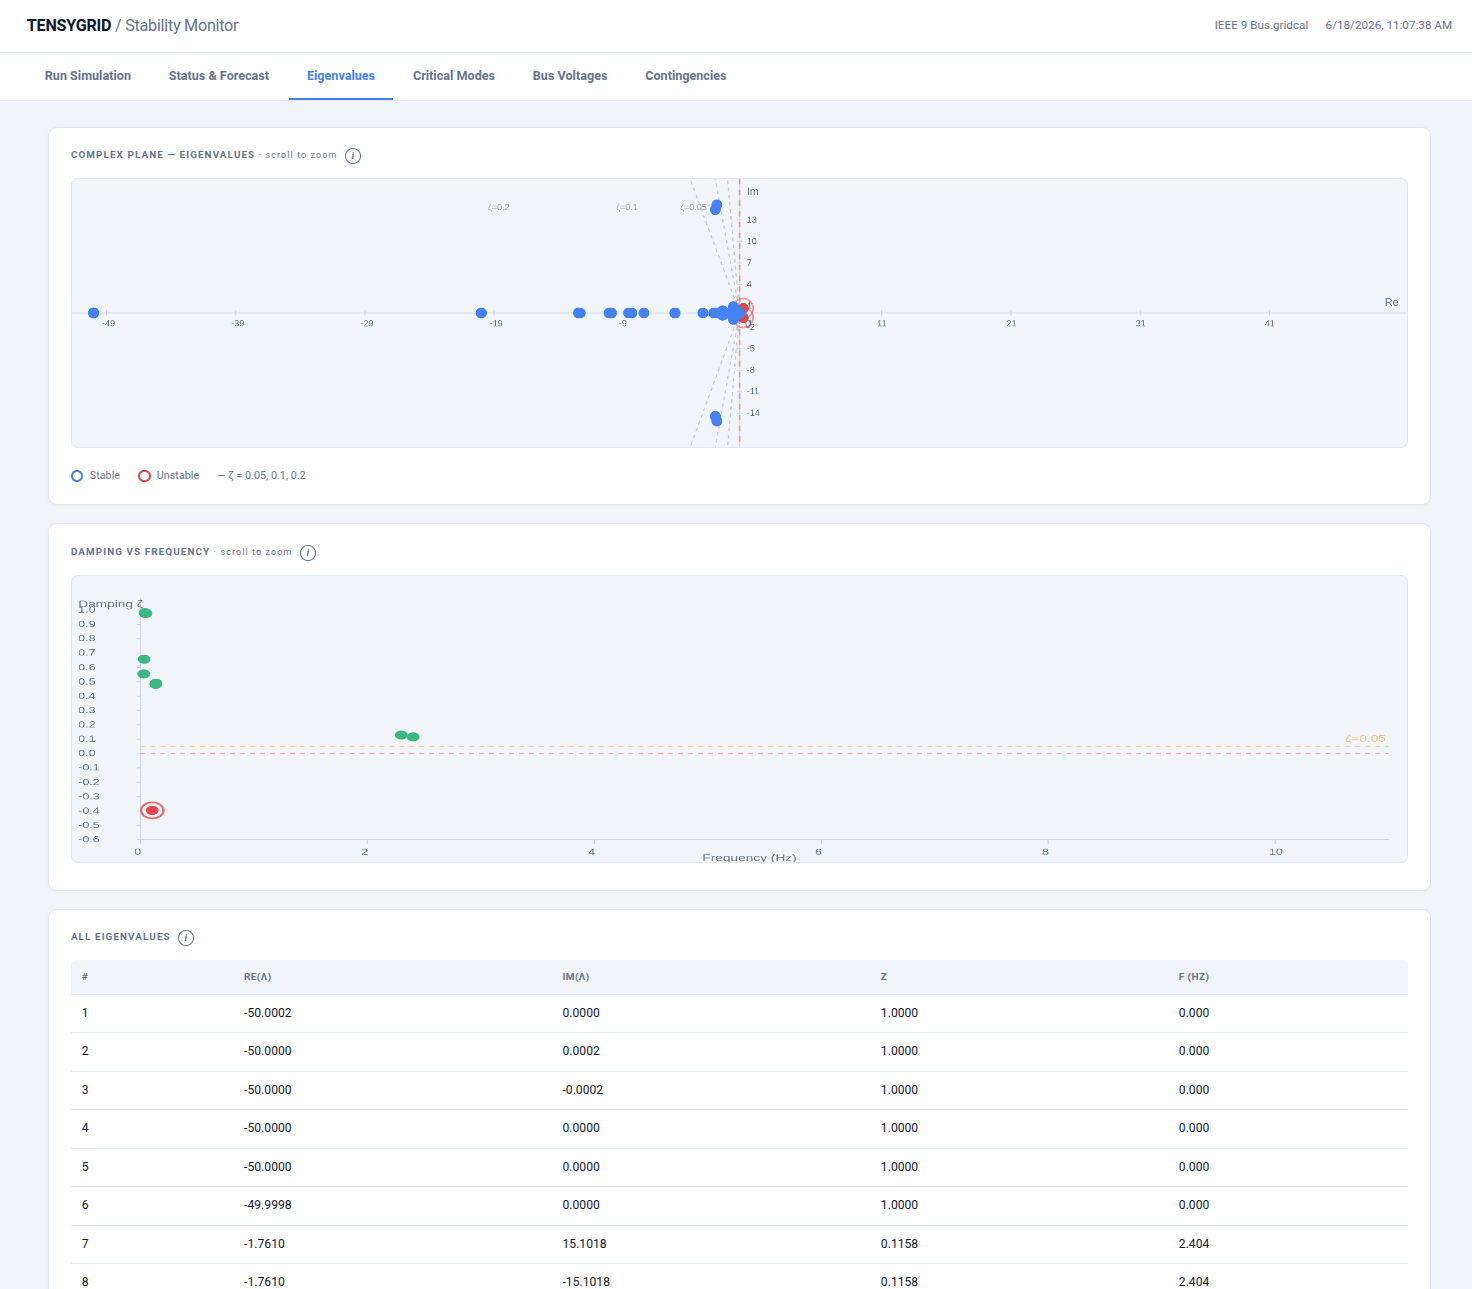
\includegraphics[width=0.7\textwidth]{pictures/UC-03.eigenvalues.png}
          \caption[UC-02: Eigenvalue analysis.]{UC-02: Eigenvalue analysis. The operator explores the eigenvalue distribution in the complex plane from the Eigenvalues tab.}
        \end{figure}

  \item[GUI interaction.] The \textbf{Status} tab is designed as a control-room dashboard. Colour-coded status badges draw the operator's attention to abnormal conditions without relying on animated traffic-light graphics. All metrics are displayed in large-format cards for quick scanning. The eigenvalue canvas of the \textbf{Eigenvalues} tab supports interactive zoom and pan via mouse or touch gestures. The damping plot and table are synchronised with the same data set and update when a different analysis result is loaded.
  \item[Expected result.] The operator obtains a clear answer to the question \textit{``Is the grid stable''?} together with enough context (topology, metrics) and a detailed understanding of the oscillatory modes (their frequencies, damping levels, and proximity to instability) to decide whether further investigation is needed. If the status is yellow or red, the operator is expected to proceed to UC-03 for detailed diagnosis of the critical modes, and uses this view to evaluate the effectiveness of remedial measures in contingency scenarios (UC-05).
\end{description}

% ---------------------------------------------------------------------------
\subsection{UC-03: Identification and diagnosis of critical oscillatory modes}
% ---------------------------------------------------------------------------

\begin{description}
  \item[Actor.] Stability engineer or control designer.
  \item[Objective.] Identify the least-damped oscillation modes and determine which state variables (generators, controls, components) contribute most to each mode.
  \item[Preconditions.] An analysis (UC-01) has been completed. Eigenvalues have been computed.
  \item[Theoretical basis.] Each eigenvalue corresponds to an oscillation mode that is a specific combination of perturbations in the state vector. The modal participation factor is defined as
        \[
          p_{ki}=\frac{v_{ki}\,(\mathbf{w}_k^{\top}\mathbf{E})_i}{\mathbf{w}_k^{\top}\mathbf{E}\,\mathbf{v}_k},
        \]
        where $\mathbf{v}_k$ and $\mathbf{w}_k$ are the right and left eigenvectors of the pencil $\lambda\mathbf{E}\mathbf{x}=\mathbf{A}\mathbf{x}$ (with $\mathbf{A}\mathbf{v}_k=\lambda_k\mathbf{E}\mathbf{v}_k$, $\mathbf{w}_k^{\top}\mathbf{A}=\lambda_k\mathbf{w}_k^{\top}\mathbf{E}$), $v_{ki}=\mathbf{e}_i^{\top}\mathbf{v}_k$ and $(\mathbf{w}_k^{\top}\mathbf{E})_i=\mathbf{w}_k^{\top}\mathbf{E}\,\mathbf{e}_i$~\cite{tzounas2019modal}. The GUI displays normalised magnitudes
        \[
          \bar{p}_{ki}=\frac{\lvert p_{ki}\rvert}{\sum_{j}\lvert p_{kj}\rvert},
        \]
        which sum to 100\% per mode. A large $\bar{p}_{ki}$ indicates that the $k$-th mode is strongly associated with the $i$-th state, making it a primary candidate for intervention (PSS retuning, FACTS placement).
  \item[Possible bottlenecks.] In sparse computations of the eigenvalues is difficult to compute their corresponding left and right eigenvectors that are both needed for this UC.
  \item[Main flow.]
        \begin{enumerate}[before=\leavevmode, leftmargin=*]
          \item The operator navigates to the \textbf{Critical Modes} tab.
          \item A table lists the modes with the lowest damping ratios, sorted from most to least critical. Each row shows the mode index, real part, imaginary part, frequency, damping ratio, and a stability badge.
          \item The operator clicks on a mode row to expand its \textbf{participation factors}.
          \item An inline bar chart displays the relative participation of each state variable: bars are proportional to the magnitude of the participation factor, and the state variable name is shown alongside.
          \item State variables associated with the same physical device (e.g., generator speed $\Delta\omega$, rotor angle $\Delta\delta$, AVR states) are visually grouped.
          \item The operator can identify which generators or components dominate the mode, helping to target power system stabiliser (PSS) tuning or FACTS placement at the most effective locations.
        \end{enumerate}

        \begin{figure}[H]
          \centering
          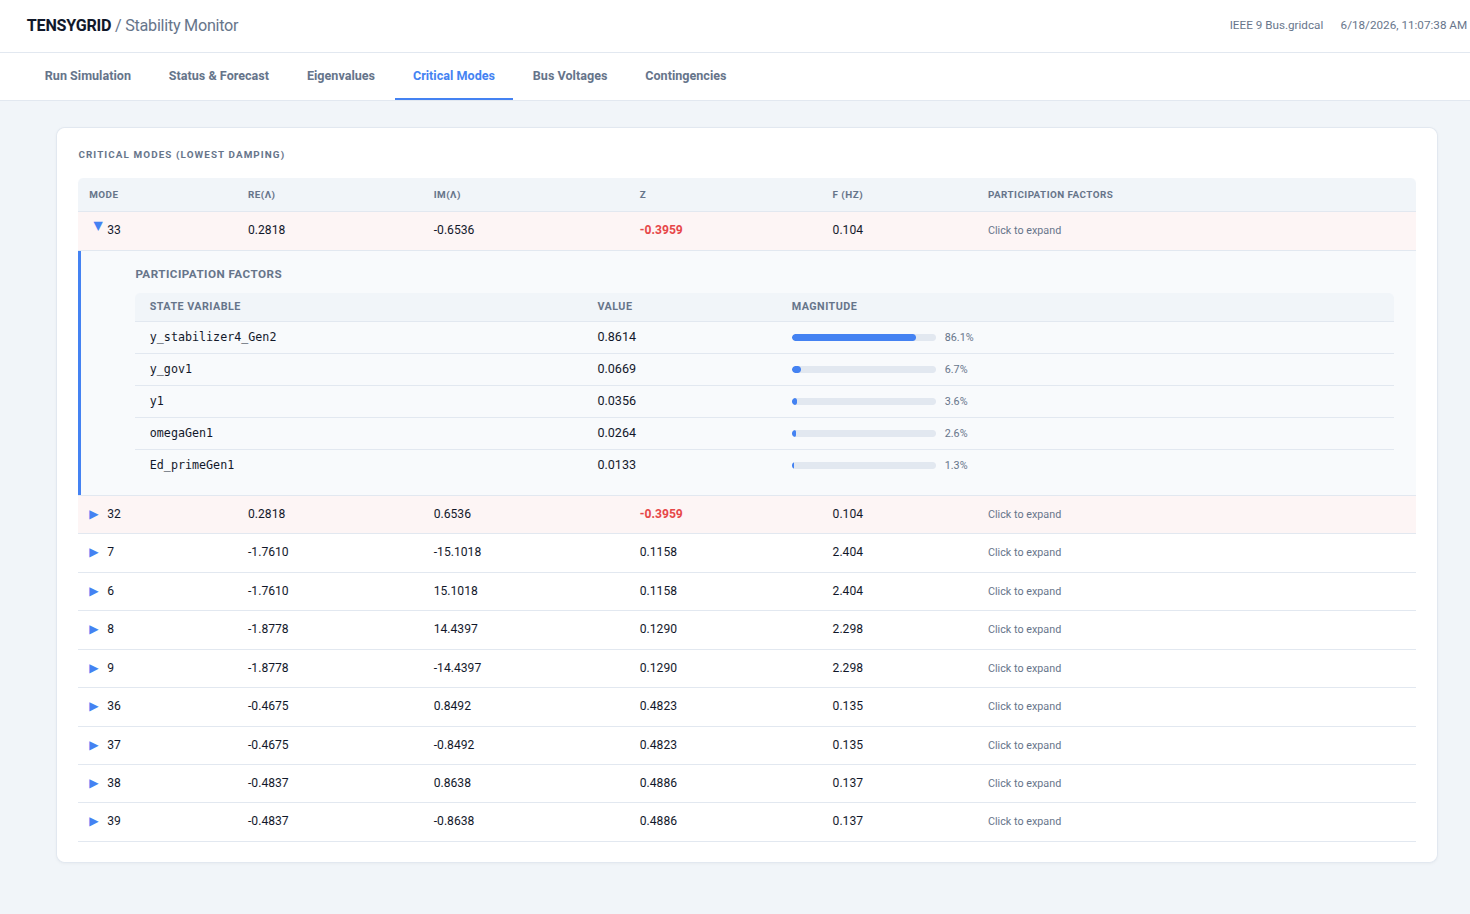
\includegraphics[width=0.7\textwidth]{pictures/UC-04.critical_modes.png}
          \caption[UC-03: Critical modes.]{UC-03: Critical modes. The operator identifies the least-damped oscillation modes.}
        \end{figure}
  \item[GUI interaction.] Participation factors are rendered as horizontal bar charts inside expandable table rows. The expansion is animated. The operator can collapse a row and expand another to compare participation profiles across different modes.
  \item[Expected result.] The operator learns \textit{which physical components are responsible for each critical oscillation}. For example, Mode 3 with $\zeta = 0.02$ at 1.2 Hz may show strong participation from Generator 7's speed and AVR states, indicating that retuning the PSS at that generator would be the most effective mitigation. This directly informs the decisions proposed in next use cases.
\end{description}

% ---------------------------------------------------------------------------
\subsection{UC-04: Assessment of bus voltage profiles and operating limit violations}
% ---------------------------------------------------------------------------

\begin{description}
  \item[Actor.] Network operator.
  \item[Objective.] Verify that the voltage magnitudes obtained from the power-flow solution are within acceptable operating limits.
  \item[Preconditions.] An analysis (UC-01) has been completed and the power-flow solution is available.
  \item[Theoretical basis.] The power-flow solution provides the steady-state voltage magnitude and angle at each bus of the network. The per-unit voltage magnitude $V_\mathrm{p.u.}$ is compared against operational limits: normal operating range (e.g.\ $0.95$--$1.05$ p.u.) and emergency limits (e.g.\ $0.90$--$1.10$ p.u.). Buses outside the normal range but within emergency limits are flagged as WARNING; buses beyond emergency limits indicate a severe violation. UC-04 does not perform an iMTI calculation independently. It reuses the operating-point power flow already required by UC-01 and complements the eigenvalue-based assessment, because a system can be small-signal stable while exhibiting unacceptable voltage profiles.
  \item[Main flow.]
        \begin{enumerate}[before=\leavevmode, leftmargin=*]
          \item The operator navigates to the \textbf{Bus Voltages} tab.
          \item A table lists every bus in the network with its name (or index) and its voltage magnitude in per-unit (p.u.).
          \item Each bus row carries a colour-coded status badge:
                \begin{itemize}[before=\leavevmode, leftmargin=*]
                  \item \textbf{OK} (green) | voltage is within the normal operating range (e.g., $0.95$--$1.05$ p.u.).
                  \item \textbf{WARNING} (orange) | voltage is outside the normal range but within emergency limits (e.g., $0.90$--$1.10$ p.u.).
                \end{itemize}
          \item Buses with WARNING status are flagged for operator attention. The operator can sort the table by voltage magnitude to quickly locate under-voltage or over-voltage buses.
        \end{enumerate}

        \begin{figure}[H]
          \centering
          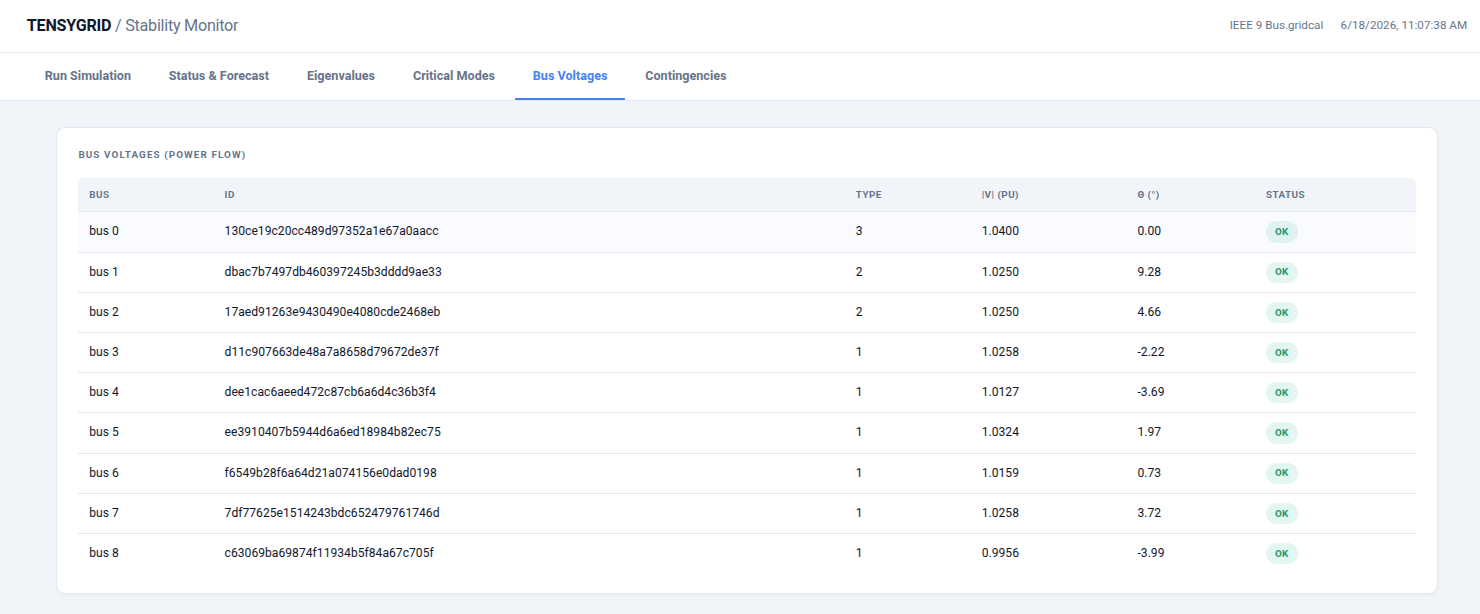
\includegraphics[width=0.7\textwidth]{pictures/UC-05.bus_voltages.png}
          \caption[UC-04: Bus voltage assessment.]{UC-04: Bus voltage assessment. The operator validates the voltage profile under the current operating point.}
        \end{figure}
  \item[GUI interaction.] The bus voltage table is a scrollable table with sortable columns. The OK/WARNING badges use the same colour semantics as the stability traffic lights, maintaining visual consistency across the interface.
  \item[Expected result.] The operator obtains a quick validation of the voltage profile under the current operating point. Buses with voltage excursions are highlighted, prompting further investigation into reactive power support, tap-changer settings, or load behaviour.
\end{description}



% ---------------------------------------------------------------------------
\subsection{UC-05: Identification of stability risks under $N-1$ contingencies}
% ---------------------------------------------------------------------------

\begin{description}
  \item[Actor.] Network operator or planning engineer.
  \item[Objective.] Evaluate the impact of a single-element outage (generator, line, or load) on the small-signal stability of the grid.
  \item[Preconditions.]
        \begin{itemize}[before=\leavevmode, leftmargin=*]
          \item A base-case analysis (UC-01) has been completed and serves as the pre-contingency reference.
          \item The grid model contains the values of the element to be removed.
        \end{itemize}
  \item[Theoretical basis.] For each selected outage, the affected device is changed from \texttt{active} to \texttt{inactive}. A new power flow determines the post-contingency equilibrium, after which the iMTI descriptor matrices and eigenvalues are recomputed. The use case is therefore not a conventional $N-1$ power-flow check alone: its TenSyGrid contribution is the comparison of pre- and post-contingency small-signal stability margins and critical modes.
  \item[Main flow.]
        \begin{enumerate}[before=\leavevmode, leftmargin=*]
          \item The operator navigates to the \textbf{Contingencies} tab.
          \item The operator selects the contingency type from a dropdown: \textbf{Generator}, \textbf{Line}, or \textbf{Load}.
          \item A second dropdown is populated with the available elements of the selected type (e.g., "Generator 0", "Line 3"). The operator selects the specific element to be removed.
          \item The operator clicks the \textbf{Analyse Contingency} button.
          \item The backend launches the contingency analysis script, which removes the selected element from the grid model, re-computes the power flow and the small-signal stability, and returns the post-contingency eigenvalues.
          \item The results are displayed as a side-by-side comparison: two complex-plane eigenvalue plots (pre-contingency vs.~post-contingency) sharing the same axis scales, plus a summary table listing the contingency type, the element removed, and the change in stability margin.
          \item The tool generates \textbf{automatic recommendations} based on the observed change:
                \begin{itemize}[before=\leavevmode, leftmargin=*]
                  \item If the system becomes unstable: ``Consider installing PSS at the most participating generators or adding a STATCOM/SVC near the affected bus''
                  \item If damping degrades below the 5\% threshold: ``Low-damped modes detected; evaluate PSS retuning or FACTS placement''
                  \item If the stability margin decreases significantly: ``Re-dispatch generation or reinforce the affected corridor to recover margin''
                \end{itemize}
          \item The operator can repeat the analysis for different elements to explore multiple $N-1$ scenarios. A \textbf{Stop} button is available to cancel a running contingency analysis if it takes too long.
        \end{enumerate}
        \begin{figure}[H]
          \centering
          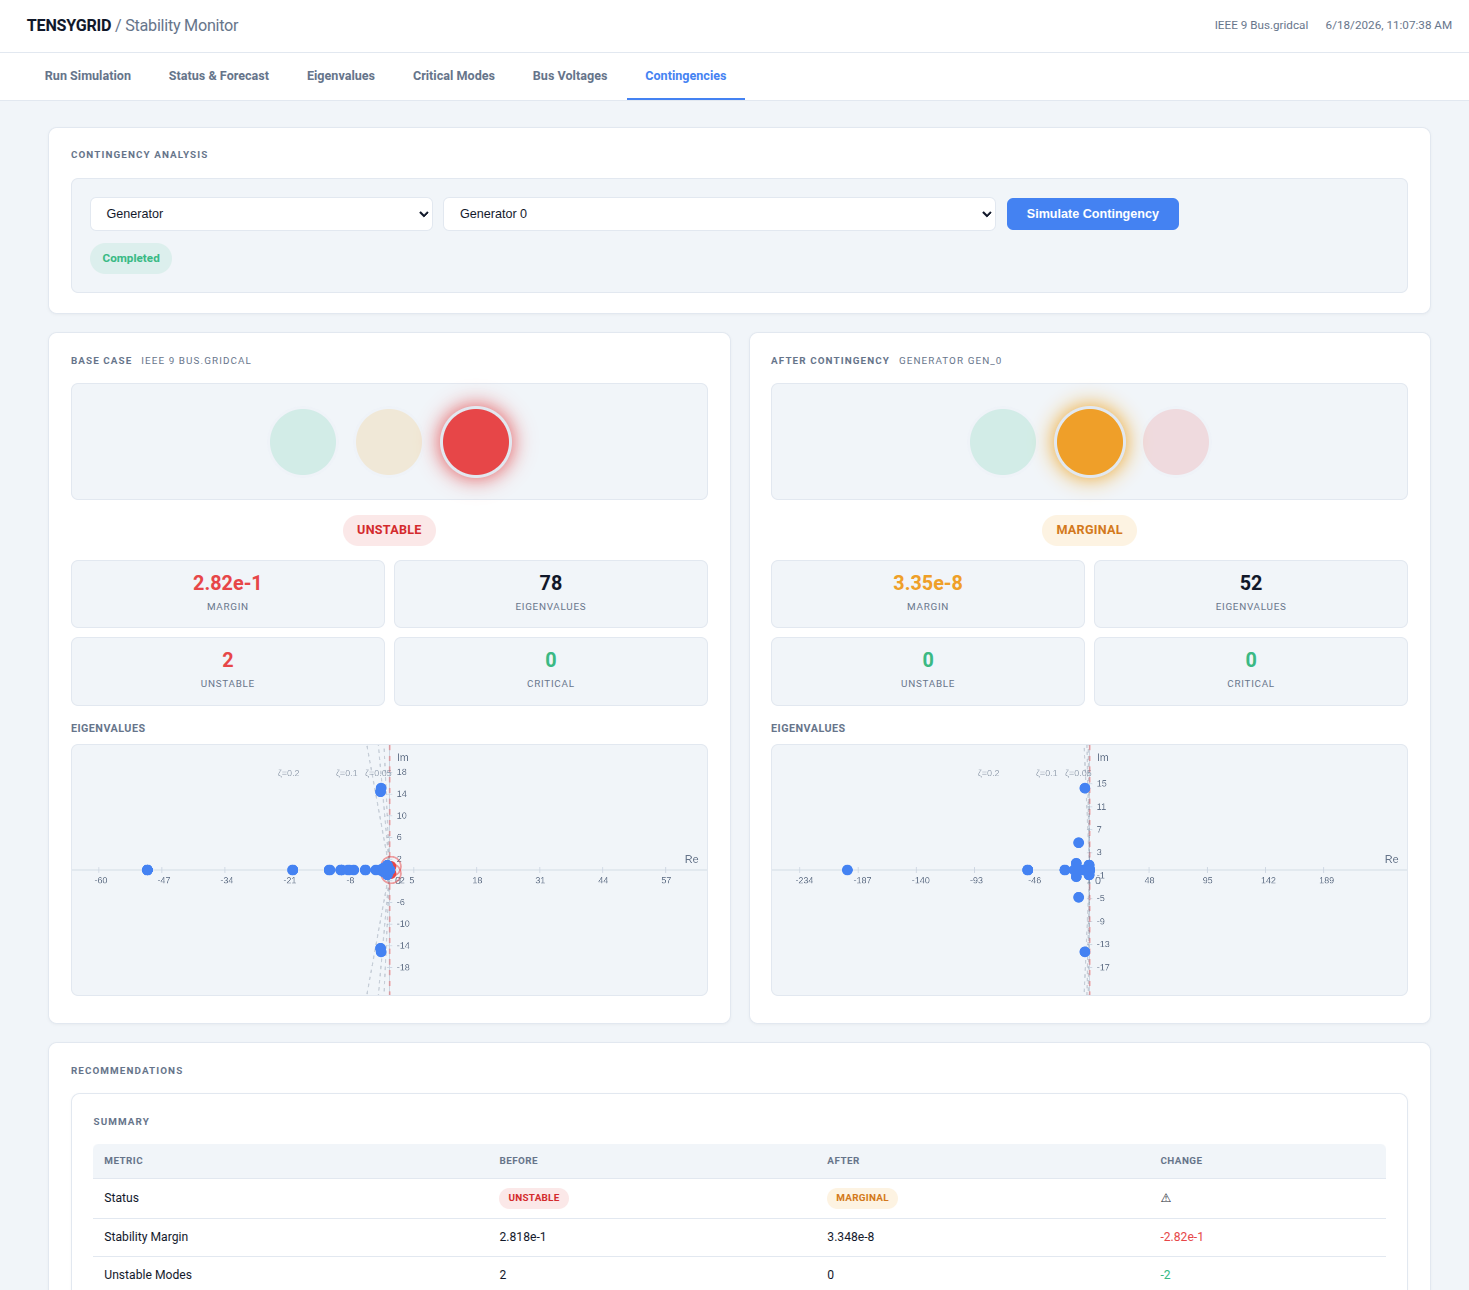
\includegraphics[width=0.7\textwidth]{pictures/UC-06.contingencies.png}
          \caption[UC-05: Contingency analysis.]{UC-05: Contingency analysis. The operator evaluates the impact of different contingencies on system stability.}
        \end{figure}
  \item[GUI interaction.] The Contingencies tab uses a three-column layout: controls on the left, eigenvalue comparison in the centre, and recommendations on the right. The before/after plots share the same axis scales for direct visual comparison.
  \item[Expected result.] The operator determines whether the grid remains stable under the selected $N-1$ contingency. If instability or marginal stability is detected, the operator receives targeted, actionable recommendations. This use case supports transmission planning studies and operational security assessment, enabling the operator to identify critical contingencies and plan mitigation measures.
\end{description}
